% Intended LaTeX compiler: xelatex
\documentclass[11pt]{article}
\usepackage{graphicx}
\usepackage{grffile}
\usepackage{longtable}
\usepackage{wrapfig}
\usepackage{rotating}
\usepackage[normalem]{ulem}
\usepackage{amsmath}
\usepackage{textcomp}
\usepackage{amssymb}
\usepackage{capt-of}
\usepackage{hyperref}
\author{Jacob Debel}
\date{}
\title{Lineær regression\\\medskip
\large Matematik grundforløb}
\hypersetup{
 pdfauthor={Jacob Debel},
 pdftitle={Lineær regression},
 pdfkeywords={},
 pdfsubject={},
 pdfcreator={Emacs 27.2 (Org mode 9.4.4)}, 
 pdflang={Danish}}
\begin{document}

\maketitle



\section*{Punkter og rette linjer}
\label{sec:orgd36e194}

\subsection*{Hvad ved i forvejen?}
\label{sec:org2b89100}

\begin{itemize}
\item Hvor mange punkter skal man kende, for at kunne tegne en ret linje?
\item 2
\end{itemize}

\begin{center}
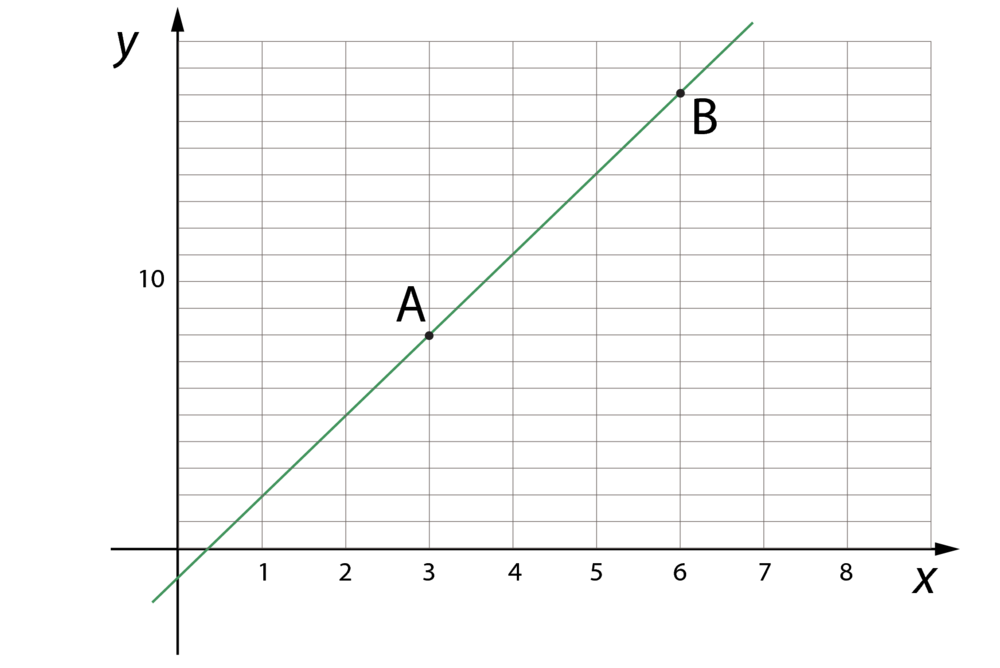
\includegraphics[width=.9\linewidth]{img/csm_haeldningen_a_ca5c3a73d5_2019-09-05_09-23-37.png}
\end{center}

\subsection*{Hvad hvis der er flere end to punkter?}
\label{sec:org8230d13}

\begin{center}
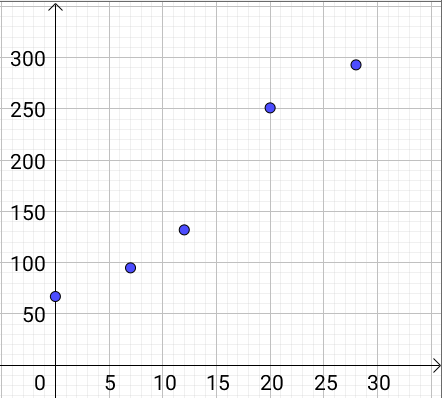
\includegraphics[width=.9\linewidth]{img/screenshot_2019-09-05_09-29-54.png}
\end{center}

\subsection*{Tegn i hånden}
\label{sec:org1815f5c}

Antal oddere i Danmark

\begin{center}
\begin{tabular}{lrrrrr}
Årstal, x & 1984 (0) & 1991 (7) & 1996 (12) & 2004 (20) & 2012 (28)\\
\hline
Observationer, y & 67 & 95 & 132 & 251 & 293\\
\end{tabular}
\end{center}

\begin{itemize}
\item Indtegn datasættet på tegnet papir i hånden.
\item Indtegn selv den \emph{bedst mulige} rette linje.
\end{itemize}

\begin{center}
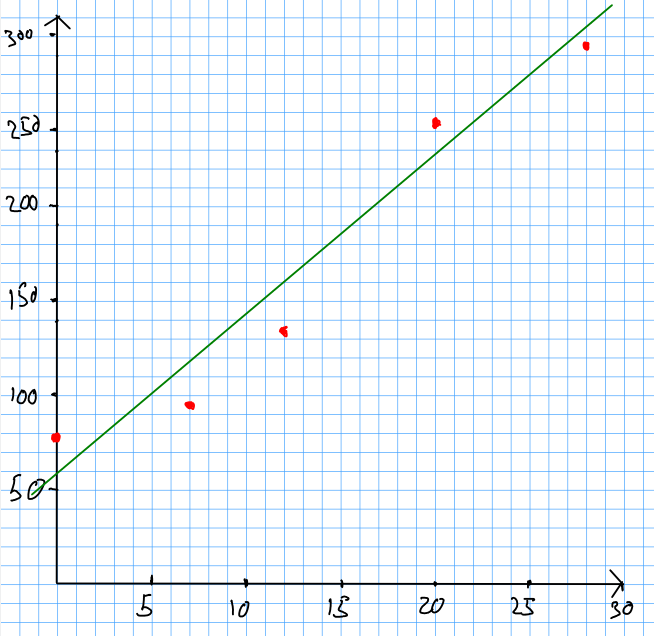
\includegraphics[width=.9\linewidth]{img/screenshot_2019-09-05_09-49-25.png}
\end{center}

\subsection*{Konklusion}
\label{sec:org95415f9}

\begin{itemize}
\item Grafen går måske ikke igennem nogen af punkterne.
\item Grafen skal være så tæt på alle punkterne som muligt.
\end{itemize}

\subsection*{Interaktiv øvelse}
\label{sec:orgd56344a}
\url{https://matbhtx.systime.dk/?id=c12359}

\begin{center}
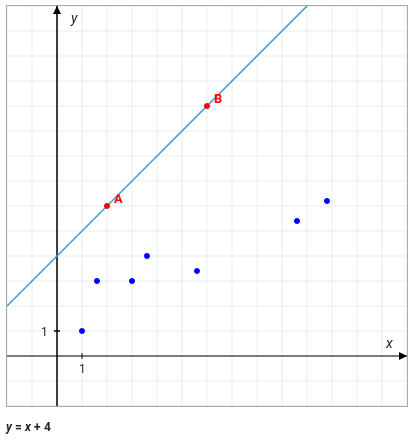
\includegraphics[width=.9\linewidth]{img/screenshot_2019-09-05_09-54-19.png}
\end{center}

\section*{Mindste kvadraters metode}
\label{sec:org449302c}

\subsection*{Den bedst mulige rette linje}
\label{sec:org7e42469}

\begin{center}
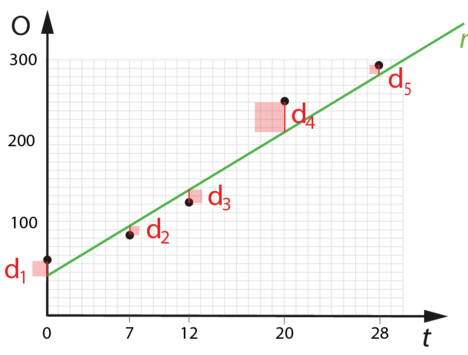
\includegraphics[width=.9\linewidth]{img/screenshot_2019-09-05_10-23-36.png}
\end{center}

\begin{center}
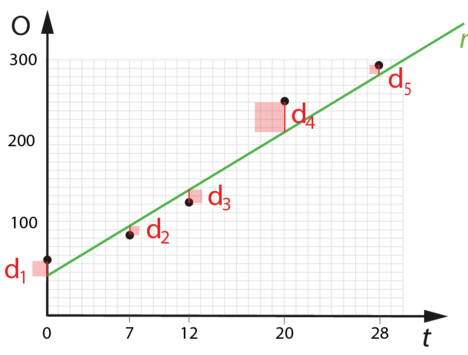
\includegraphics[width=.9\linewidth]{img/screenshot_2019-09-05_10-23-36.png}
\end{center}
\begin{itemize}
\item Undersøger den lodrette afstand mellem de kendte punkter og en given ret linje.
\item \emph{Residualer}
\item \emph{Kvadratiske afvigelser}
\item Summen af alle de kvadratiske afvigelser, skal være så lille som muligt. $$D=d_1^2 + d_2^2 + d_3^2 + d_4^2 + d_5^2$$
\end{itemize}

\subsection*{Prøv det selv}
\label{sec:orge4805aa}

Mindste\_kvadraters\_metode.ggb på lectio

\begin{center}
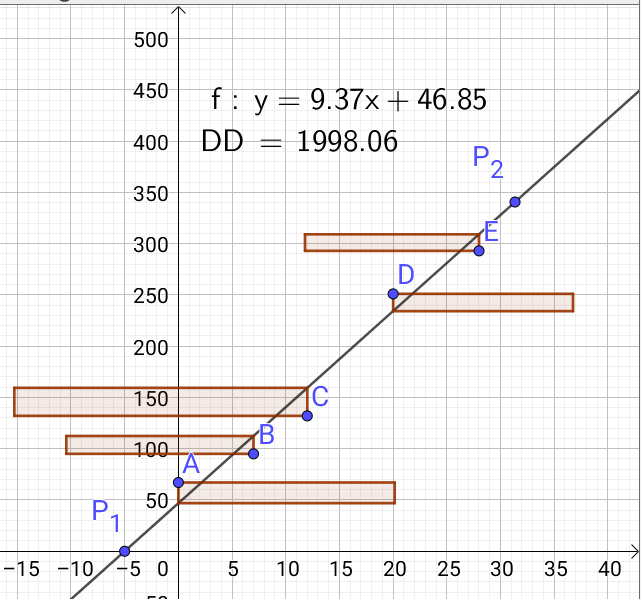
\includegraphics[width=.9\linewidth]{img/screenshot_2019-09-05_10-39-25.png}
\end{center}

\begin{itemize}
\item Flyt på \(P_1\) og \(P_2\).
\item Få \(DD\) til at blive så lille som muligt.
\end{itemize}

\subsection*{Få Geogebra til at gøre det}
\label{sec:org634a361}

Indtast følgende i \emph{input}-feltet:

\begin{itemize}
\item \texttt{liste1=\{A,B,C,D,E\}} (Opret en liste med punkter)
\item \texttt{FitLinje(liste1)} (Finder den bedste rette linje)
\end{itemize}

\section*{Hvor godt passer det så?}
\label{sec:org44a4a10}

\subsection*{Korrelationskoeffiecenten, \(r\)}
\label{sec:org18da27b}

\begin{center}
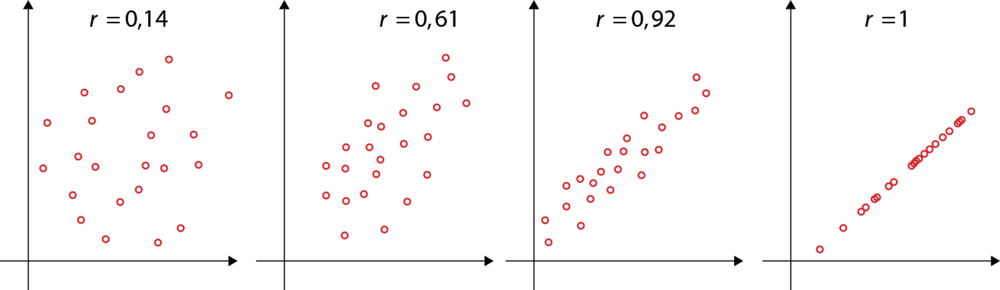
\includegraphics[width=.9\linewidth]{img/csm_123_rverdi_9467cbf6c5_2019-09-05_10-53-12.png}
\end{center}

\begin{center}
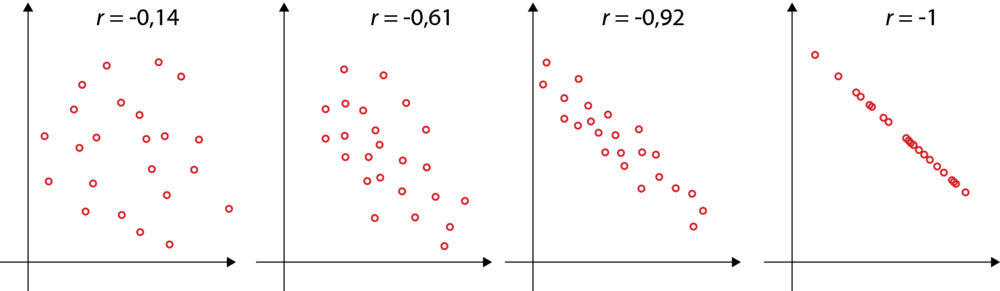
\includegraphics[width=.9\linewidth]{img/csm_124_rverdi_spejl_b07c3ce819_2019-09-05_10-53-33.png}
\end{center}

\begin{itemize}
\item Kommando i geogebra: \texttt{PMCC(<liste med punkter>)} (say what!?)
\end{itemize}

\subsection*{Forklaringsgraden, \(r^2\)}
\label{sec:orgd12597b}

\begin{itemize}
\item \(0 \leq r^2 \leq 1\)
\item \(r^2 = 1\) - Perfekt \emph{fit}.
\item \(r^2 = 0\) - Det dårligste fit overhovedet.
\item \(r^2 > 0.99\) - Godt lineært fit.
\item \(0.95 < r^2< 0.99\) - Rimeligt lineært fit.
\item Kommando i geogebra: 

\texttt{Rkvadreret(<liste med punkter>, <funktion>)}
\end{itemize}

\subsection*{Opgave}
\label{sec:org0e94b0e}

\begin{center}
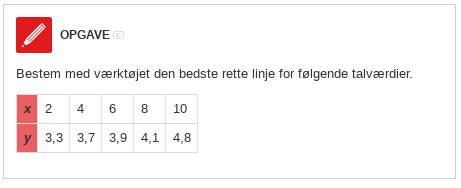
\includegraphics[width=.9\linewidth]{img/screenshot_2019-09-05_11-08-46.png}
\end{center}
\begin{itemize}
\item Indsæt punkter i geogebra (\texttt{(2,3.3)} i inputfeltet etc)
\item Opret liste med punkter (\texttt{liste1=\{A,B\}} og alle de andre punkter også)
\item Fit en ret linje (\texttt{fitlinje(liste1)})
\item Find forklaringsgraden (\texttt{Rkvadreret(liste1,f)})
\end{itemize}

\subsection*{Flere opgaver}
\label{sec:orga626851}
\url{https://matbhtx.systime.dk/index.php?id=1295}

\begin{center}
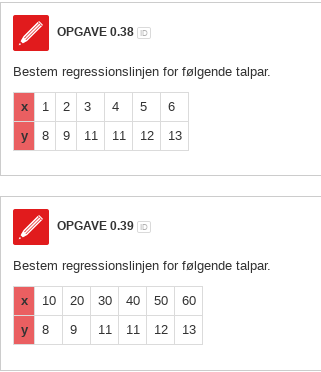
\includegraphics[width=.9\linewidth]{img/screenshot_2019-09-05_11-18-40.png}
\end{center}
\begin{center}
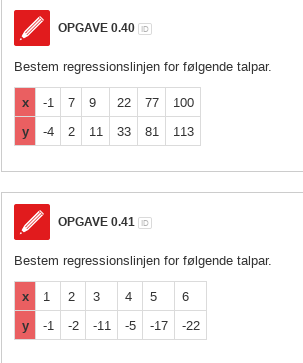
\includegraphics[width=.9\linewidth]{img/screenshot_2019-09-05_11-18-52.png}
\end{center}
\begin{center}
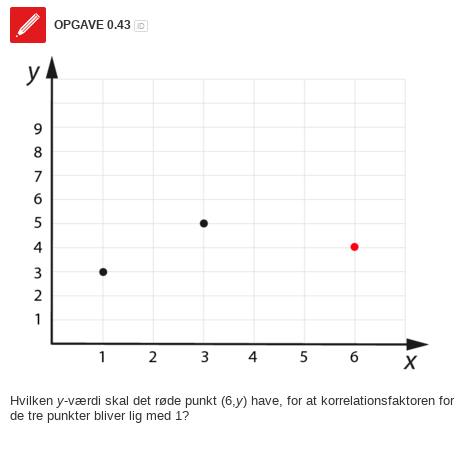
\includegraphics[width=.9\linewidth]{img/screenshot_2019-09-05_11-19-49.png}
\end{center}

\begin{center}
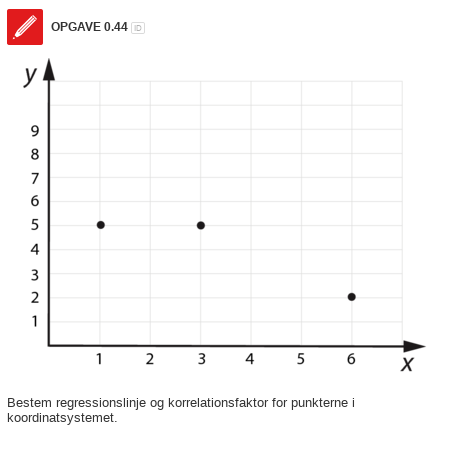
\includegraphics[width=.9\linewidth]{img/screenshot_2019-09-05_11-20-04.png}
\end{center}

\section*{Backup slides}
\label{sec:orga708c40}

\subsection*{Hvis man skal regne det hele i hånden}
\label{sec:org926368c}

\begin{center}
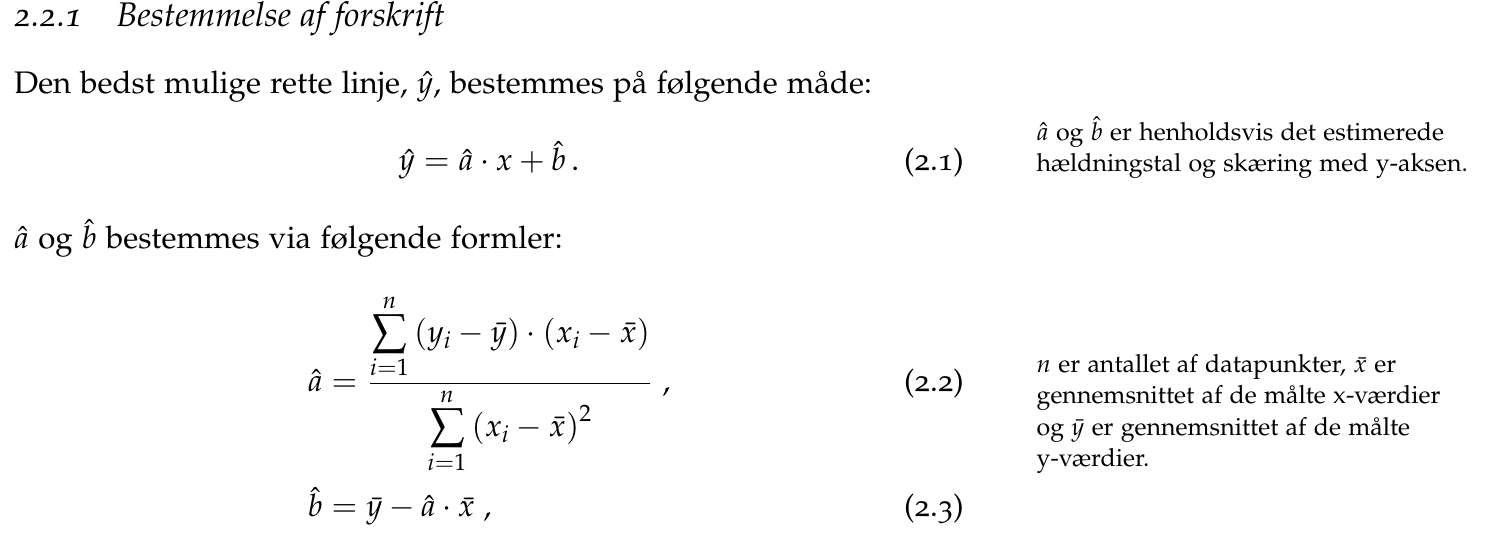
\includegraphics[width=.9\linewidth]{img/screenshot_2019-09-05_11-35-40.png}
\end{center}

\begin{center}
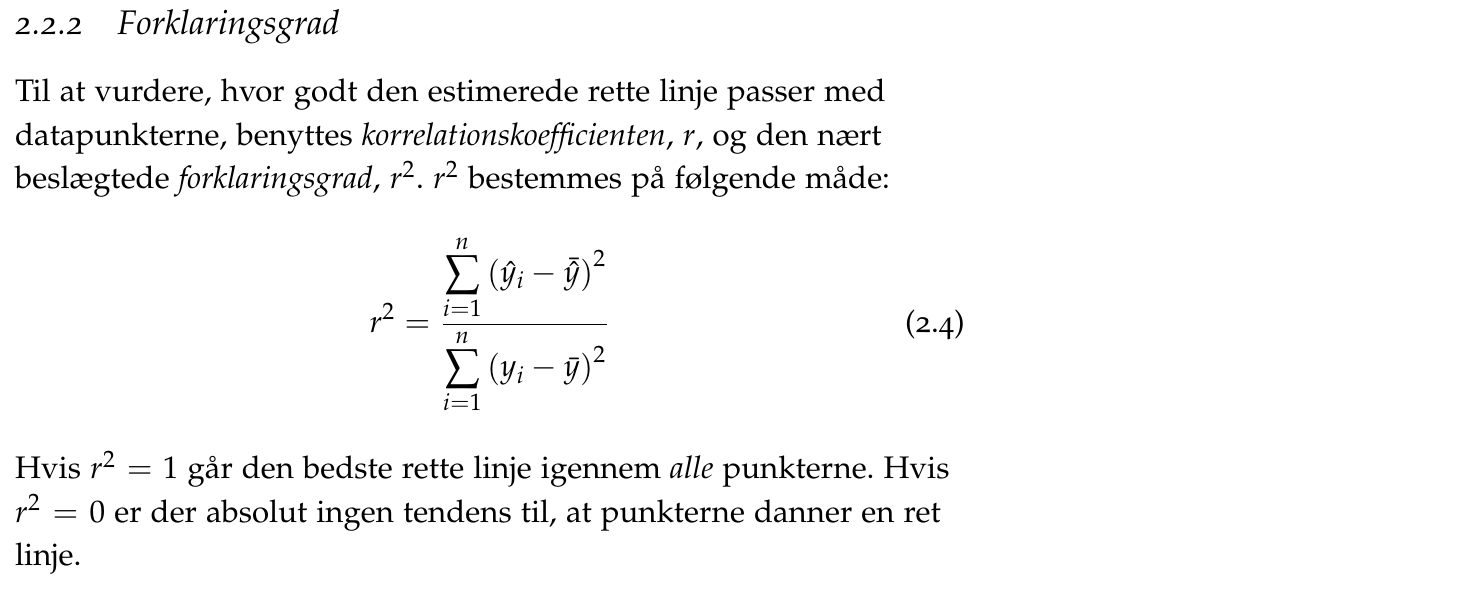
\includegraphics[width=.9\linewidth]{img/screenshot_2019-09-05_11-37-21.png}
\end{center}
\end{document}